Web-sovellusten yleistyessä törmätään yhä useammin käyttäjän tunnistautumisen ongelmaan. Sovelluksen tarjoaja haluaa, että vain tietyillä käyttäjillä on pääsy järjestelmään. Tämä vaatii käyttäjän tunnistamisen, ts. käyttäjä on se, joka väittää olevansa. Kun web-sovelluksia on yhä enemmän, käyttäjän tunnistamiseen käytettäviä valtuutustietoja (credentials) syntyy useita, jolloin käyttäjän täytyy muistaa useita käyttäjätunnus/salasana-pareja.

Samaan ongelmaan törmätään usein myös intranet-palveluissa, kun niiden arkkitehtuuria viedään palveluperustaiseen suuntaan. Tällöin jokaisen palvelun täytyy pystyä tunnistamaan käyttäjä, jotta hänelle voidaan näyttää käyttöoikeuksien mukaan sisältöä. Intranetin palveluilla voi olla oma käyttäjätietokanta, joka synkronoidaan päätietokannan kanssa, jolloin yksittäisellä palvelulla on ajantasainen tieto käyttäjän oikeudesta käyttää palvelua. Tässä tapauksessa ongelmallista on, että käyttäjän tunnukset ja salasanat siirtyvät useaan järjestelmään, joka heikentää järjestelmän tietoturvaa \cite{nisti}. Jos taas eri intranetin palveluihin luodaan oma tunnus, syntyy uusi muistettava tunnus/salasana-pari.

Palveluille voidaan avata pääsy organisaation käyttäjähallintaan, jolloin palveluun pääsy edellyttää, että käyttäjän syöttämä tunnus/salasana-pari löytyy organisaation käyttäjähallinnasta. Tämä voi olla järjestelmän ylläpitäjän näkökulmasta ongelmallista, sillä käyttäjäkanta sisältää tietoja, joiden ei haluta päätyvän ulkopuolisten käsiin. Yhtenä ratkaisuna on esitetty keskitettyä tunnistautumispalvelua, jolla on pääsy käyttäjähallintaan ja jota vasten yksittäiset web-sovellukset tunnistavat käyttäjät \cite{nisti}. Kuvassa \ref{johdanto_kuva} on esitetty arkkitehtuurikuva järjestelmästä, joka käyttää tunnistatumispalvelua käyttäjän tunnistamiseen.

\begin{figure}[ht]
\centering
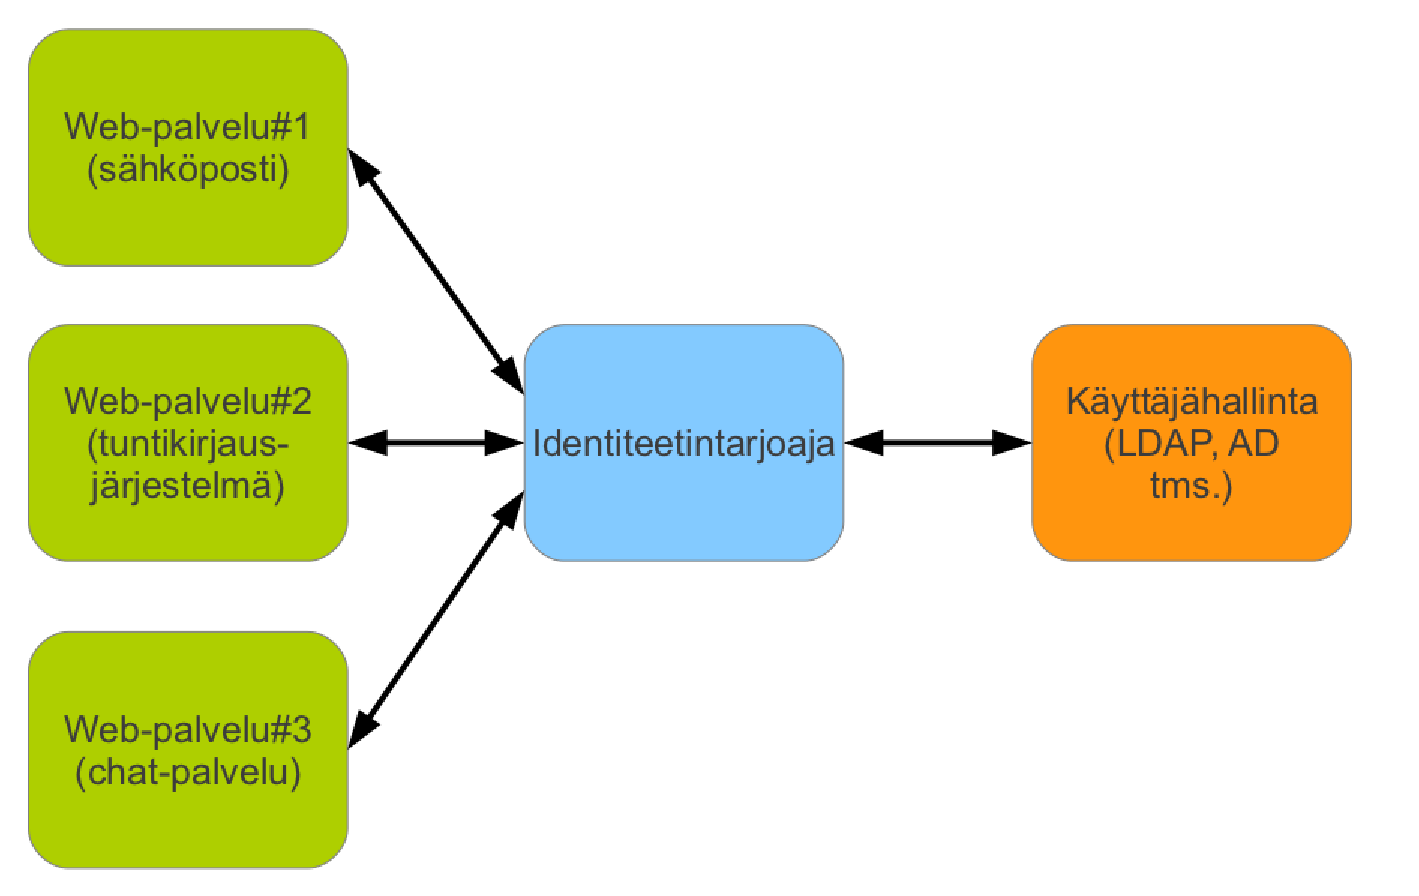
\includegraphics[width=.7\textwidth]{misc/johdanto_kuva.eps}
\caption{Arkkitehtuurikuva järjestelmässä, joka käyttää keskitettyä tunnistautumispalvelua.}%
\label{johdanto_kuva}
\end{figure}

Tässä tutkielmassa paneudutaan mainittuun ongelmakenttään ja tutkitaan ratkaiseeko keskitetty tunnistautumispalvelu esitetyt ongelmat ja millaisia mahdollisia uusia ongelma se tuo tullessaan. Pohditaan myös millaisia etuja erillisestä tunnistautumispalvelusta on verrattuna suoraan integraatioon käyttäjähallintaan. Etuja ja haittoja punnitaan järjestelmän ylläpitäjän, käyttäjän ja web-sovellusohjelmoijan näkökulmasta.

Tutkielmassa ei keskitytä kaikille avoimiin tunnistautumispalveluihin (kuten Facebook tai Google), vaan organisaatioihin, joilla on oma käyttäjähallinta. Esimerkki tällaisesta organisaatiosta on Helsingin Yliopisto, jolla on oma Active Directory -käyttäjähallinta \cite{tietotekniikkaa}. Myös monet yritykset ylläpitävät omaa käyttäjähallintaa esimerkiksi LDAP-järjestelmässä tai keskitetyssä tietokannassa. Esimerkkinä hyötyjä ja haittoja punnittaessa käytetään Helsingin Yliopistoa, mutta myös muunlaiset organisaatiot huomioidaan, mikäli se on perusteltua.

Tutkielma jakautuu kahteen osaan. Luvuissa 2, 3 ja 4 käsitellään ongelmakenttään liittyvää teoriaa. Luvussa 2 esitellään web-sovellukset, erityisesti palveluperustaiset web-sovellukset. Luvussa 3 käydään läpi käyttäjän tunnistautumisen tekniikoita ja ongelmakenttää. Luvussa 4 käsitellään keskitettyä tunnistautumista palveluperustaisissa arkkitehtuureissa. Luvut ...
